\documentclass[pdflatex]{sn-jnl}
 \renewcommand{\textfraction}{.002}
\renewcommand{\floatpagefraction}{.995}
\setcounter{totalnumber}{5}
\renewcommand{\topfraction}{.995}

\usepackage[numbers,square]{natbib}
\bibliographystyle{spbasic_u}

\usepackage[noend,ruled,vlined]{algorithm2e}
\newcommand\mycommfont[1]{\footnotesize\ttfamily{#1}}
\SetCommentSty{mycommfont}


\usepackage{graphicx}%
\usepackage{multirow}%
\usepackage{amsmath,amssymb,amsfonts}%
\usepackage{amsthm}%
\usepackage{mathrsfs}%
\usepackage[title]{appendix}%
\usepackage{xcolor}%
\usepackage{textcomp}%
\usepackage{manyfoot}%
\usepackage{booktabs}%
\usepackage{placeins}
\usepackage{listings}%
\usepackage{mathtools}
\usepackage{subcaption}
\usepackage{xr}
\usepackage{bm}
%% CUSTOM PACKAGES
%\usepackage[linesnumbered,ruled,vlined]{algorithm2e}
\usepackage{hyperref}
\usepackage{array}
\usepackage{tabularx}
\usepackage{tikz}
\usetikzlibrary{shapes.geometric}
%\usetikzlibrary{3d,perspective}
%\usetikzlibrary{shapes.geometric, arrows.meta, positioning}
\usepackage{booktabs} % For better table lines
\usepackage[version=4]{mhchem} 
\usepackage{enumitem}
\usepackage{algorithm2e}
%\usepackage{arydshln}

%%%%%%%%%%%%%%%%%%%%%%%%%%%%%%%%%%%%%%%%%%%%%%%%%%%%%%%%%%%%%%%%%%%%%%%%%%%

%% as per the requirement new theorem styles can be included as shown below
\theoremstyle{thmstyleone}%
\newtheorem{theorem}{Theorem}%  meant for continuous numbers
\newtheorem{corollary}[theorem]{Corollary}% 
\newtheorem{proposition}[theorem]{Proposition}%
\newtheorem{lemma}[theorem]{Lemma}% 
\newtheorem{conjecture}[theorem]{Conjecture}%
\newtheorem{observation}[theorem]{Observation}%
%
\makeatletter
\newtheoremstyle{examplesty}% Numbered
{18pt plus2pt minus1pt}% Space above
{18pt plus2pt minus1pt}% Space below
{\normalfont}% Body font
{0pt}% Indent amount
{\bfseries}% Theorem head font
{.}% Punctuation after theorem head
{.5em}% Space after theorem headi
{\thmname{#1}\thmnumber{\@ifnotempty{#1}{ }{#2}}%
  \thmnote{ {\the\thm@notefont(#3)}}}% Theorem head spec (can be left empty, meaning `normal')
\makeatother
\theoremstyle{examplesty}%
\newtheorem{example}{Example}%
%\newtheorem{remark}{Remark}%
%
\theoremstyle{thmstylethree}%
\newtheorem{definition}[theorem]{Definition}%

\newenvironment{mainitem}[2]{\medskip\par\noindent%
  \textbf{#1~M\ref{#2}.}}{\par}


%%%%% SOME LOW LEVEL STUFF NEEDED FOR SPECIAL SYMBOLS
\makeatletter
\def\moverlay{\mathpalette\mov@rlay}
\def\mov@rlay#1#2{\leavevmode\vtop{%
    \baselineskip\z@skip \lineskiplimit-\maxdimen
    \ialign{\hfil$\m@th#1##$\hfil\cr#2\crcr}}}
\newcommand{\charfusion}[3][\mathord]{
  #1{\ifx#1\mathop\vphantom{#2}\fi
    \mathpalette\mov@rlay{#2\cr#3}
  }
  \ifx#1\mathop\expandafter\displaylimits\fi}
\DeclareRobustCommand\bigop[1]{%
  \mathop{\vphantom{\sum}\mathpalette\bigop@{#1}}\slimits@
}
\newcommand{\bigop@}[2]{%
  \vcenter{%
    \sbox\z@{$#1\sum$}%
    \hbox{\resizebox{\ifx#1\displaystyle.9\fi\dimexpr\ht\z@+\dp\z@}{!}{$\m@th#2$
}}%
  }%
}
\makeatother
%%%%% END LOWLEVEL USER DEFINITION

\newcommand{\cupdot}{\charfusion[\mathbin]{\cup}{\cdot}}
\DeclareMathOperator{\bigcupdot}{\charfusion[\mathop]{\bigcup}{\cdot}}
% \DeclareMathOperator{\Aut}{Aut}
% \DeclareMathOperator{\orb}{orb}
\newcommand{\whatever}{\mbox{\,.\,}}
\newcommand{\king}{K}
\newcommand{\queen}{\mathbf{Q}}
\newcommand{\princess}{\mathbf{P}}
\newcommand{\lord}{L}
\newcommand{\food}{\ensuremath{\mathbf{F}}}
\newcommand{\SM}{S}
\newcommand{\block}[0]{\mathbf{B}}
\newcommand{\closure}[2]{\mathscr{C}_{#1}(#2)}
\newcommand{\cl}[0]{c}
\newcommand{\CR}[0]{\mathcal{R}}
\newcommand{\C}[1]{\mathit{#1}}
\newcommand{\FR}[0]{\mathbf{R}}
%\newcommand{\F}[1]{\mathbf{#1}}
\newcommand{\fr}[0]{\mathbf{r}}
\newcommand{\net}[1]{\hat{#1}}
\newcommand{\RAF}[0]{\mathbf{R}'}
\newcommand{\sgen}{g}
\newcommand{\rgen}{\gamma}
\newcommand{\RGraph}[0]{\mathcal{R}}
\newcommand{\PO}[0]{d}
\newcommand{\POR}[0]{\mathscr{R}}
\newcommand{\POX}[0]{\mathscr{X}}
\newcommand{\cat}{\mathbf{C}}
\newcommand{\ceducts}{\mathcal{E}}
\newcommand{\cproducts}{\mathcal{P}}
\newcommand{\feducts}{\mathbf{E}}
\newcommand{\fproducts}{\mathbf{P}}
\newcommand{\ORCID}[1]{}
\DeclareMathOperator{\suck}{succ}
\newcommand{\Code}[1]{\texttt{\upshape{#1}}}
\newcommand{\pfad}[0]{\ensuremath{\mathbf{P}}}
\newcommand{\stack}[0]{\ensuremath{\mathbf{T}}}
\newcommand{\child}{\pmb{\kappa}}

\definecolor{middlegreen}{RGB}{0,128,0}
\definecolor{royalpurple}{RGB}{85,26,139}
\newcommand{\NEW}[1]{\begingroup\color{blue}#1\endgroup}
\newcommand{\TODO}[1]{\begingroup\color{red}#1\endgroup}
\newcommand{\PFS}[1]{\begingroup\color{blue}#1\endgroup}
\newcommand{\holy}[1]{\begingroup\color{royalpurple}#1\endgroup}
\newcommand{\TG}[1]{\begingroup\color{green}#1\endgroup}
\newcommand{\NV}[1]{\begingroup\color{teal}#1\endgroup}
\newcommand{\OLD}[1]{\begingroup\tiny\color{gray}#1\endgroup}

% Linenumbers for debugging
\usepackage{lineno}
\linenumbers
\raggedbottom

%%%%%%%%%%%%%%%%%%%%%%%%%%%%%%%%%%%%%%%%%%%%%%%%%%%%%%%%%%%%%%%%%%%
%%%%%%%%%%%%%%%%%%%%%%%%%%%%%%%%%%%%%%%%%%%%%%%%%%%%%%%%%%%%%%%%%%%
%%%%%%%%%%%%%%%%%%%%%%%%%%%%%%%%%%%%%%%%%%%%%%%%%%%%%%%%%%%%%%%%%%%

\externaldocument[M-]{RAFCores}

\begin{document}

\title{RAF-Cores - Supplement} 

%% comment: 

\author*[1,4]{\fnm{Richard} \sur{Golnik}}\email{richard@bioinf.uni-leipzig.de}
\ORCID{0000-0002-8582-5006} 

\author[1]{\fnm{Thomas} \sur{Gatter}}\email{thomas@bioinf.uni-leipzig.de}
\ORCID{0000-0002-5016-5191} 

\author[1]{\fnm{Wim} \sur{Hordijk}}\email{wim@worldwidewanderings.net}
\ORCID{0000-0002-0223-6194} 

\author[1,2]{\fnm{Nicola} \sur{Vassena}}\email{nicola.vassena@uni-leipzig.de}
\ORCID{0000-0001-5411-4976} 

\author[1,2,3,4,5,6,7,8,9]{\fnm{Peter F.}\sur{Stadler}}\email{studla@bioinf.uni-leipzig.de}
\ORCID{0000-0001-5567-3016}

\affil[1]{\orgdiv{Bioinformatics Group, Department of Computer Science}
  \orgname{Leipzig University}, \orgaddress{\street{H{\"a}rtelstra{\ss}e 16–18},
    \postcode{D-04107} \city{Leipzig}, \country{Germany}}} 

\affil[2]{\orgdiv{Interdisciplinary Center for Bioinformatics}
	\orgaddress{\orgname{Leipzig University}, \postcode{D-04107}
	 \city{Leipzig}, \country{Germany}}}  
	 
\affil[3]{\orgdiv{Center for Scalabale Data Analytics and Artificial Intelligence},
  \orgaddress{\orgname{Leipzig University}, \postcode{D-04107}
    \city{Leipzig}, \country{Germany}}} 

\affil[4]{\orgdiv{Zuse School for Embedded and Composite Artificial Intelligence (SECAI)}
   \orgaddress{\orgname{Leipzig University}, \postcode{D-04107}
    \city{Leipzig}, \country{Germany}}}

\affil[5]{\orgname{Max Planck Institute for Mathematics in the Sciences},
  \orgaddress{\street{Inselstra{\ss}e 22}, \postcode{D-04103}
    \city{Leipzig}, \country{Germany}}}

\affil[6]{\orgdiv{Department of Theoretical Chemistry}, \orgname{University
    of Vienna}, \orgaddress{\street{W{\"a}hringerstra{\ss}e 17},
    \postcode{A-1090} \city{Wien}, \country{Austria}}}

\affil[7]{\orgdiv{Facultad de Ciencias}, \orgname{Universidad National de
    Colombia}, \orgaddress{\city{Bogot{\'a}}, \country{Colombia}}}

\affil[8]{\orgdiv{Center for non-coding RNA in Technology and Health},
  \orgname{University of Copenhagen}, \orgaddress{\street{Ridebanevej 9},
    \postcode{DK-1870} \city{Frederiksberg}, \country{Denmark}}}

\affil[9]{\orgname{Santa Fe Institute}, \orgaddress{\street{1399 Hyde Park
      Rd.}, \city{Santa Fe}, \state{NM} \postcode{87501}, \country{USA}}}


% Contact information of the corresponding author
%\corr{Correspondence:
%  Richard Golnik, richard@bioinf.uni-leipzig.de; Tel.: +49-341-97-16626}



%\abstract{
%}

%%%%%%%%%%%%%%%%%%%%%%%%%%%%%%%%%%%%%%%%%%
\maketitle

\section{Glossary on Graph Theory}\label{sec:Glossary}

\paragraph{Graphs} A graph $G=(V,E)$ is a tuple composed of a set of vertices and 
a set of edges. Edges encode the adjacency of elements $u,v\in V$, i.e., $\{u,v\}\in E$ 
whenever $u$ is adjacent to $v$. We write $V(G)$ and $E(G)$ for the set of vertices 
and edges of a given graph $G$.
 
\paragraph{Directed Graphs} In a directed graph $G\coloneqq (V,E)$, edges are ordered 
pairs instead of unordered pairs, and $(u,v) \in E$ whenever there is an edge from $u$ to 
$v$. The underyling undirected graph of $G$ is the graph $G_{\circ} \coloneqq (V, E_{\circ})$ with
$E_{\circ}\coloneqq \{ \{u,v\} \ \vert \ (u,v) \in E(G) \}$.

\paragraph{Subgraphs} A subgraph of a (directed) graph $G$, denoted as $G'\subseteq G$ is a graph $G=(V', E')$ 
such that $V'\subseteq V$ and $E'\subseteq E$. A subgraph \emph{induced} by a set of vertices 
$V'\subseteq V$ is the graph $G[V']\coloneqq (V', F)$ with $F\coloneqq \{ \{u,v\} \ \vert \ u,v\in V', 
\{u,v\} \in E\}$ or in the directed case $F\coloneqq \{(u,v) \ \vert \ u,v\in V', (u,v) \in E\}$.

\paragraph{Paths and Directed Paths} A (directed) path $\mathcal{P}_{v_1v_k}$ in a (directed) graph $G$ is 
a sequence of pairwise distinct vertices $(v_1,\ldots, v_k)$ such that $\{v_i, v_{i+1}\}\in E(G) \  ((v_i, v_{i+1})\in E(G)), 
1\leq i\leq k-1$.

\paragraph{(Strongly) Connected (Sub-)Graphs} A subgraph $G'\coloneqq (V', E')$ of a (directed) graph 
$G=(V,E)$ is called (strongly) connected if for any two vertices $u,v\in V'$ there is a path 
$\mathcal{P}_{uv}$, which, in the directed case, implies that there is a path from $u$ to $v$ and 
from $v$ to $u$. If $G$ is directed, then $G'\subseteq G$ is called connected if $G'_\circ$ is connected. 
If $G'$ is not connected, we may also write that $G$ is disconnected. $V'$ is called a (strongly) connected 
component if $G[V']$ is (strongly) connected and maximal, i.e., if there is no $v\in V\setminus V': V'\cup \{v\}$ 
is (strongly) connected. If $V'=V$ then we say that $G$ is (strongly) connected. 

\paragraph{Cut vertex} For a graph $G\coloneqq (V, E)$ a vertex $v\in V$ is called a cut-vertex if $G[V\setminus \{v\}]$ 
is disconnected. Accordingly, in the directed case, then $v\in V$ is a cut-vertex if $G_\circ[V\setminus \{v\}]$ is 
disconnected. 

\paragraph{Strong blocks} For a digraph $G\coloneqq (V, E)$ a strongly connected subgraph $G'\subseteq G$ is 
called a strongly connected block or strong block if it does not contain a cut-vertex.

\paragraph{Elementary circuit} An elementary circuit of length $k$ in a digraph $G\coloneqq (V,E)$ is a sequence 
of vertices $(v_1,\ldots, v_k, v_1)$ such that $(v_1,\ldots, v_k)$ is a path, $(v_k, v_1) \in E$. 

\paragraph{Digon} A digon is an elementary circuit of length $2$.

\section{RAFs}

\subsection{A \TODO{Pre}-Order on RAFs}

The easiest way to define such a partial order is by generating the set
$\closure{R'}{X'}$ iteratively. Let therefore:
\begin{equation}
  c_{\RAF}: 2^X \rightarrow 2^X, c_{\RAF}(X') \coloneqq X' \cup \{\fproducts(\fr) \subseteq X' \ \vert \ \feducts(\fr)\subseteq X'\}. 
\end{equation}
We may drop the subscript $\RAF$ whenever appropriate. In particular, we
write $c(X')$ instead of $c_{\RAF}(X')$ as well as $\closure{}{X'}$ instead
of $\closure{\RAF}{X'}$. \PFS{By construction, $c:2^X \rightarrow 2^X$ is a
  generalized closure operator, i.e., it satisfies, for all $X',X''\in 2^X$
  \begin{itemize}
  \item[(c0)] $c(\emptyset)=\emptyset$,
  \item[(c1)] $X'\subseteq X''$ implies $c(X')\subseteq c(X'')$ (isotone)
  \item[(c2)] $X\subseteq c(X')$ (extensive)
  \end{itemize}
  A set $X\subseteq X'$ is closed (w.r.t.\ $c$) if $X'=c(X')$.  Since $X$
  is finite, iterated application $c$ eventually yields a close set: to see
  this is suffices to note that by (c1) and (c2) we have $X'\subseteq
  c^k(X')\subseteq c^{k+1}(X')$ for all $k\ge 1$. Thus for every $X'\in X$,
  there is $n\in\mathbb{N}$ such that $c^{n+1}(X')=c^{n}(X')$. Moreover,
  comparison of the definitions of $c$ and $\mathscr{C}$ implies that
  $c(\mathscr{C}(X'))=\mathscr{C}(X')$, and conversely $c(X')=X'$ implies
  $X'=\mathscr{C}(X')$. Considering a finite CRS network $(X,\FR,\cat)$
  with $\food\subseteq X, \RAF\subseteq \FR$, there is $n\in\mathbb{N}$
  such that
  \begin{equation}
    \label{eq:seqLimit}
    \closure{\food} = c^k(\food) \qquad\text{for all } k\ge n 
  \end{equation}
}

The sequence $(c^k(\food))_{k\in\mathbb{N}}$ therefore defines a sequence
of reactions that can be executed in the $k$-th step, i.e., for which all
reactants are contained in the set $\cl^k(\food)$:
\begin{equation}
	d^k(X') \coloneqq \{\fr\in \RAF \ | \ \feducts(\fr)\subseteq c^k(\food)\}
\end{equation}
We can then restrict the sets obtained by $c^k(\food)$ and $d^k(\food)$ to those species and 
reactions that are not present in an ``earlier'' set $c^\ell(\food)$ and $d^\ell(\food), \ell<k$, respectively:
\begin{equation}
  \begin{split}
    X^0(\food')& \coloneqq \food \qquad X^k(\food)\coloneqq c^k(\food)\setminus \left(\bigcup_{i=0}^{k-1} c^k(\food) \right)\\
    \FR^0(\food) & \coloneqq \emptyset \qquad \FR^k(\food)\coloneqq d^k(\food) \setminus \left(\bigcup_{i=0}^{k-1} d^k(\food) \right)
  \end{split}
\end{equation}
These sequences naturally generate a partial order $\preceq$, which we make
explicit by two maps that extract for each species and reaction, the
iteration of their first appearance:
\begin{equation}\label{eq:Gen}
  \begin{split}
    \sgen&: \closure{\RAF}{\food} \rightarrow \mathbb{N}, \sgen(x)\coloneqq k \quad \text{ s. t. } x\in X^k(\PFS{\food}) \\
    \rgen&: \RAF \rightarrow \mathbb{N}, \rgen(r)\coloneqq k \quad \text{ s. t. } r\in \FR^k(\PFS{\food}). 
  \end{split}
\end{equation}
In particular, a species $x_1$ precedes a species $x_2: x_1\preceq x_2$ if and only if $\sgen(x_1) \leq \sgen(x_2)$ 
and a reaction $\fr_1$ precedes a reaction $\fr_2: \fr_1\preceq \fr_2$ if and only if $\rgen(\fr_1) \leq \rgen(\fr_2)$. We refer 
to the values of $\sgen$ and $\rgen$ as the generation of an F-reaction or metabolite. Since for some$\fr\in \FR$ all $r\in \fr$ 
share the same F-reactants, we might also define for $reactions$:
\begin{equation}
  \delta: \varphi^{-1}(\RAF)\rightarrow \mathbb{N}, \delta(r)\coloneqq
  \rgen(\fr)
\end{equation}

The partial order $\preceq$ allows us to easily observe that each species
vertex for the closure of a $\RAF$ is reachable from at least one food
molecule in $\food$ in the bipartite K{\"o}nig graph, which is restricted
to the $\closure{\RAF}{\food}$, the reactions in $\RAF$, and to those
catalyzations $\cat'$ of reactions in $\RAF\subseteq \FR$. Throughout, we
denote this graph as $\queen'\coloneqq \queen(\closure{\RAF}{\food}, \RAF,
\cat')$.


\subsection{The Binary Polymer Model}\label{sec:BinPol}

The binary polymer model is an abstract model of polymer chemistry that was introduced to argue about the probability of emergence of autocatalytic sets in random reaction networks. The set of molecules $X$ consists of all binary strings up to a maximal specified length $n$. In general, the reaction set $\FR$ consists of all possible \emph{ligation} reactions concatenating two bit strings together into a product as long as it does not exceed the maximum polymer length $n$ together with their reverse \emph{cleavage} reactions that decompose a bit string into two smaller ones. We denote the inverse of an F-reaction $\fr$ with $\overset{\leftarrow}{\fr}$. The food set $\food$ consists of all binary strings up to a given length $t$, here always $t=2$, i.e., the food set consists of the monomer and dimers. However, for some models $\FR$ is composed of ligation reactions only.

Catalysis is assigned randomly. In particular, there is a fixed probability $p$ that a given molecule (binary string) can catalyze a given F-reaction. For instances containing both ligation and cleavage, F-reactions that are the inverse of each other share the same catalysts. In other words, to create an instance of the binary model, for predetermined $n$ and $t$, each molecule-reaction pair $(x,\fr), x \in X, \fr \in \FR$ is included in the set of catalyzations $\cat(\FR)$ with probability $p$. More formally, an instance of the binary polymer model forms a CRS $\mathbf{\Phi}\coloneqq (X, \FR, \cat(\FR))$, where:
\begin{itemize}
  \item {$X = \{0,1\}^{\leq n} \text{ and } \FR \coloneqq \FR_f \cup \FR_r$} 
  \item {$\FR_f \coloneqq \{x_i + x_j \rightarrow x_i \cdot x_j : (x_i, x_j \in X) \wedge (|x_i \cdot x_j| \leq n)\}$}
  \item {$\FR_r \coloneqq \{x_i \cdot x_j \rightarrow x_i + x_j : (x_i\cdot x_j \in X)\}$} 
  \item {$\mathbb{P}[(x \in X, \fr \in \FR_f) \in \cat(\FR)] = p$}
  \item {$\mathbb{P}[(x \in X, \fr \in \FR_r) \in \cat(\FR)] = \begin{cases} 1 & \text{if} (x, \overset{\leftarrow}{\fr}) \in \cat(\FR) \\ 0 & \text{otherwise} \end{cases} $}
  \item {$\food = \{0,1\}^{\leq t}$}
\end{itemize}

\subsection{Simulation Details}

Table~\ref{tab:SimulationDetails} specifies simulation details for different instances of the binary polymer models. 
In particular, all models contributed to the generation of Fig.~\ref{fig:StrongBlocks}, while only \textit{n6\_split} 
and \textit{n6\_forw} were employed for the generation of Fig.~\ref{M-fig:irrRAFCores} and Fig.~\ref{M-fig:FoodVsNonFood}.

\begin{table}[htb]
	\caption{Specification of simulation details for irreducible RAFs from different instances of the binary polymer model. 
	Maximal polymer size is specified by $n$, while the maximum size of food molecules is specified by $t$. The 
	uniform probability for a non-food molecule to catalyze an F-reaction is given by $p$, while food species are excluded 
	from being catalysts. F-reactions are in general considered irreversible.}
	\label{tab:SimulationDetails}
	\begin{tabular}{p{1.5cm}|p{1.5cm}|p{1.5cm}|p{1.5cm}|p{1.5cm}|p{1.5cm}|p{1cm}}
	Name & n & t & p & food-catalysts & Ligation & Cleavage \\
	\hline 
	n4\_split     		& 	4 	& 	1 	& 	0.018 	& 	no 	& 	yes 		& 	yes 		\\
	n5\_forw   			& 	5  	& 	2 	& 	0.014 	& 	no 	& 	yes 		& 	no 		\\
	n5irrev 			& 	5 	& 	2 	& 	0.015 	& 	no 	& 	yes 		& 	no 		\\
	n5irrev2    		& 	5 	& 	2 	& 	0.017 	& 	no 	& 	yes 		& 	no 		\\
	n6\_split			& 	6 	& 	2 	& 	0.0025	& 	no 	& 	yes 		& 	yes		\\
	n6\_split\_red 		& 	6 	& 	2 	&	0.002	& 	no 	& 	yes 		& 	yes 		\\
	n6\_forw			& 	6 	& 	2	&      0.006	&	no 	& 	yes 		& 	no 		\\
	n7\_split			&      7	&	2	&	0.0012	&	no	& 	yes		& 	yes 		\\
	n7\_split\_red		&	7	&	2	&	0.0009	&	no	&	yes 		& 	yes		\\
	n7\_forw          		&	7	& 	2	&	0.0025	&	no	&	yes 		&	no 		\\
	n7\_forw\_red		&	7	&	2	&	0.0022	&	no	&	yes 		&	no 		\\
	n8\_split			&	8	&	2	&	0.00055	&	no	&	yes 		&	yes 		\\
	n8\_forw			&	8	&	2	&	0.0012	&	no	&	yes 		&	no 		\\
	\end{tabular}
\end{table}

\subsection{Maximal Strong Blocks}
\begin{figure}[htb]
	\vspace{-24pt}
	\begin{minipage}[c]{0.5\textwidth}
		\centering
	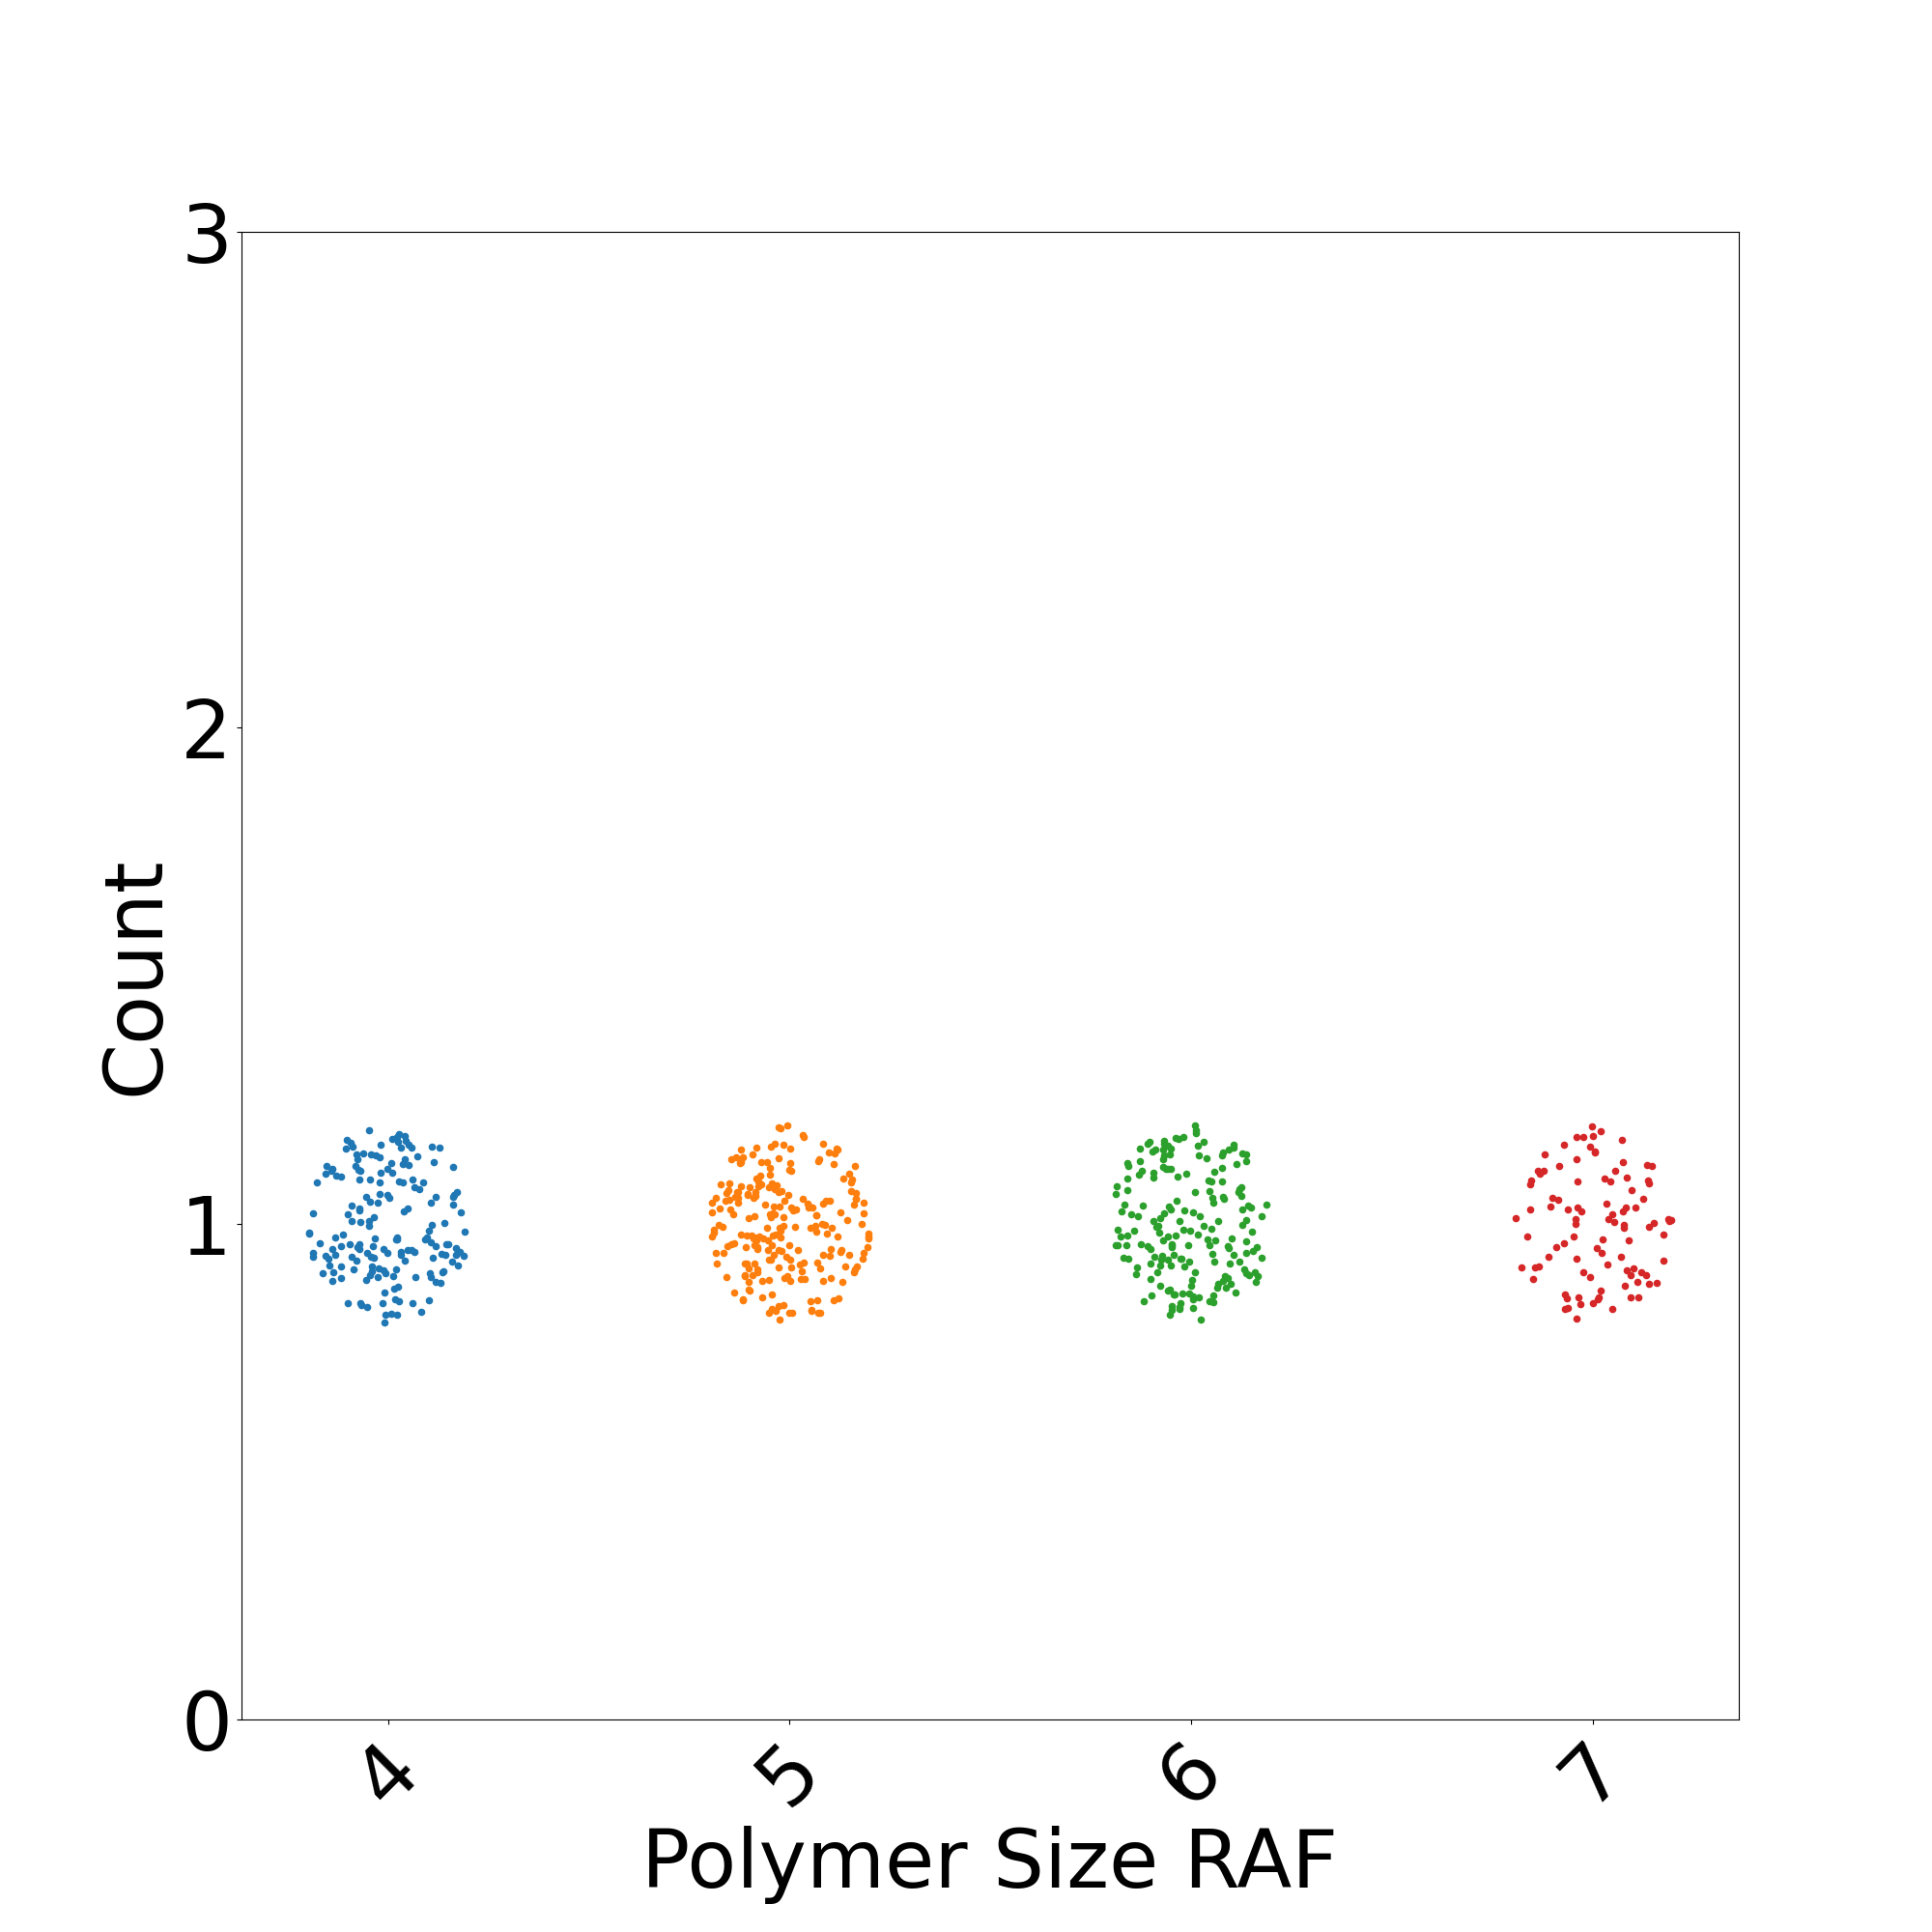
\includegraphics[width=0.8\textwidth]{./Pictures/iRAFrevStrongBlocks.png}
	\end{minipage}%
	\hfill%
	\begin{minipage}[c]{0.5\textwidth}
		\centering
		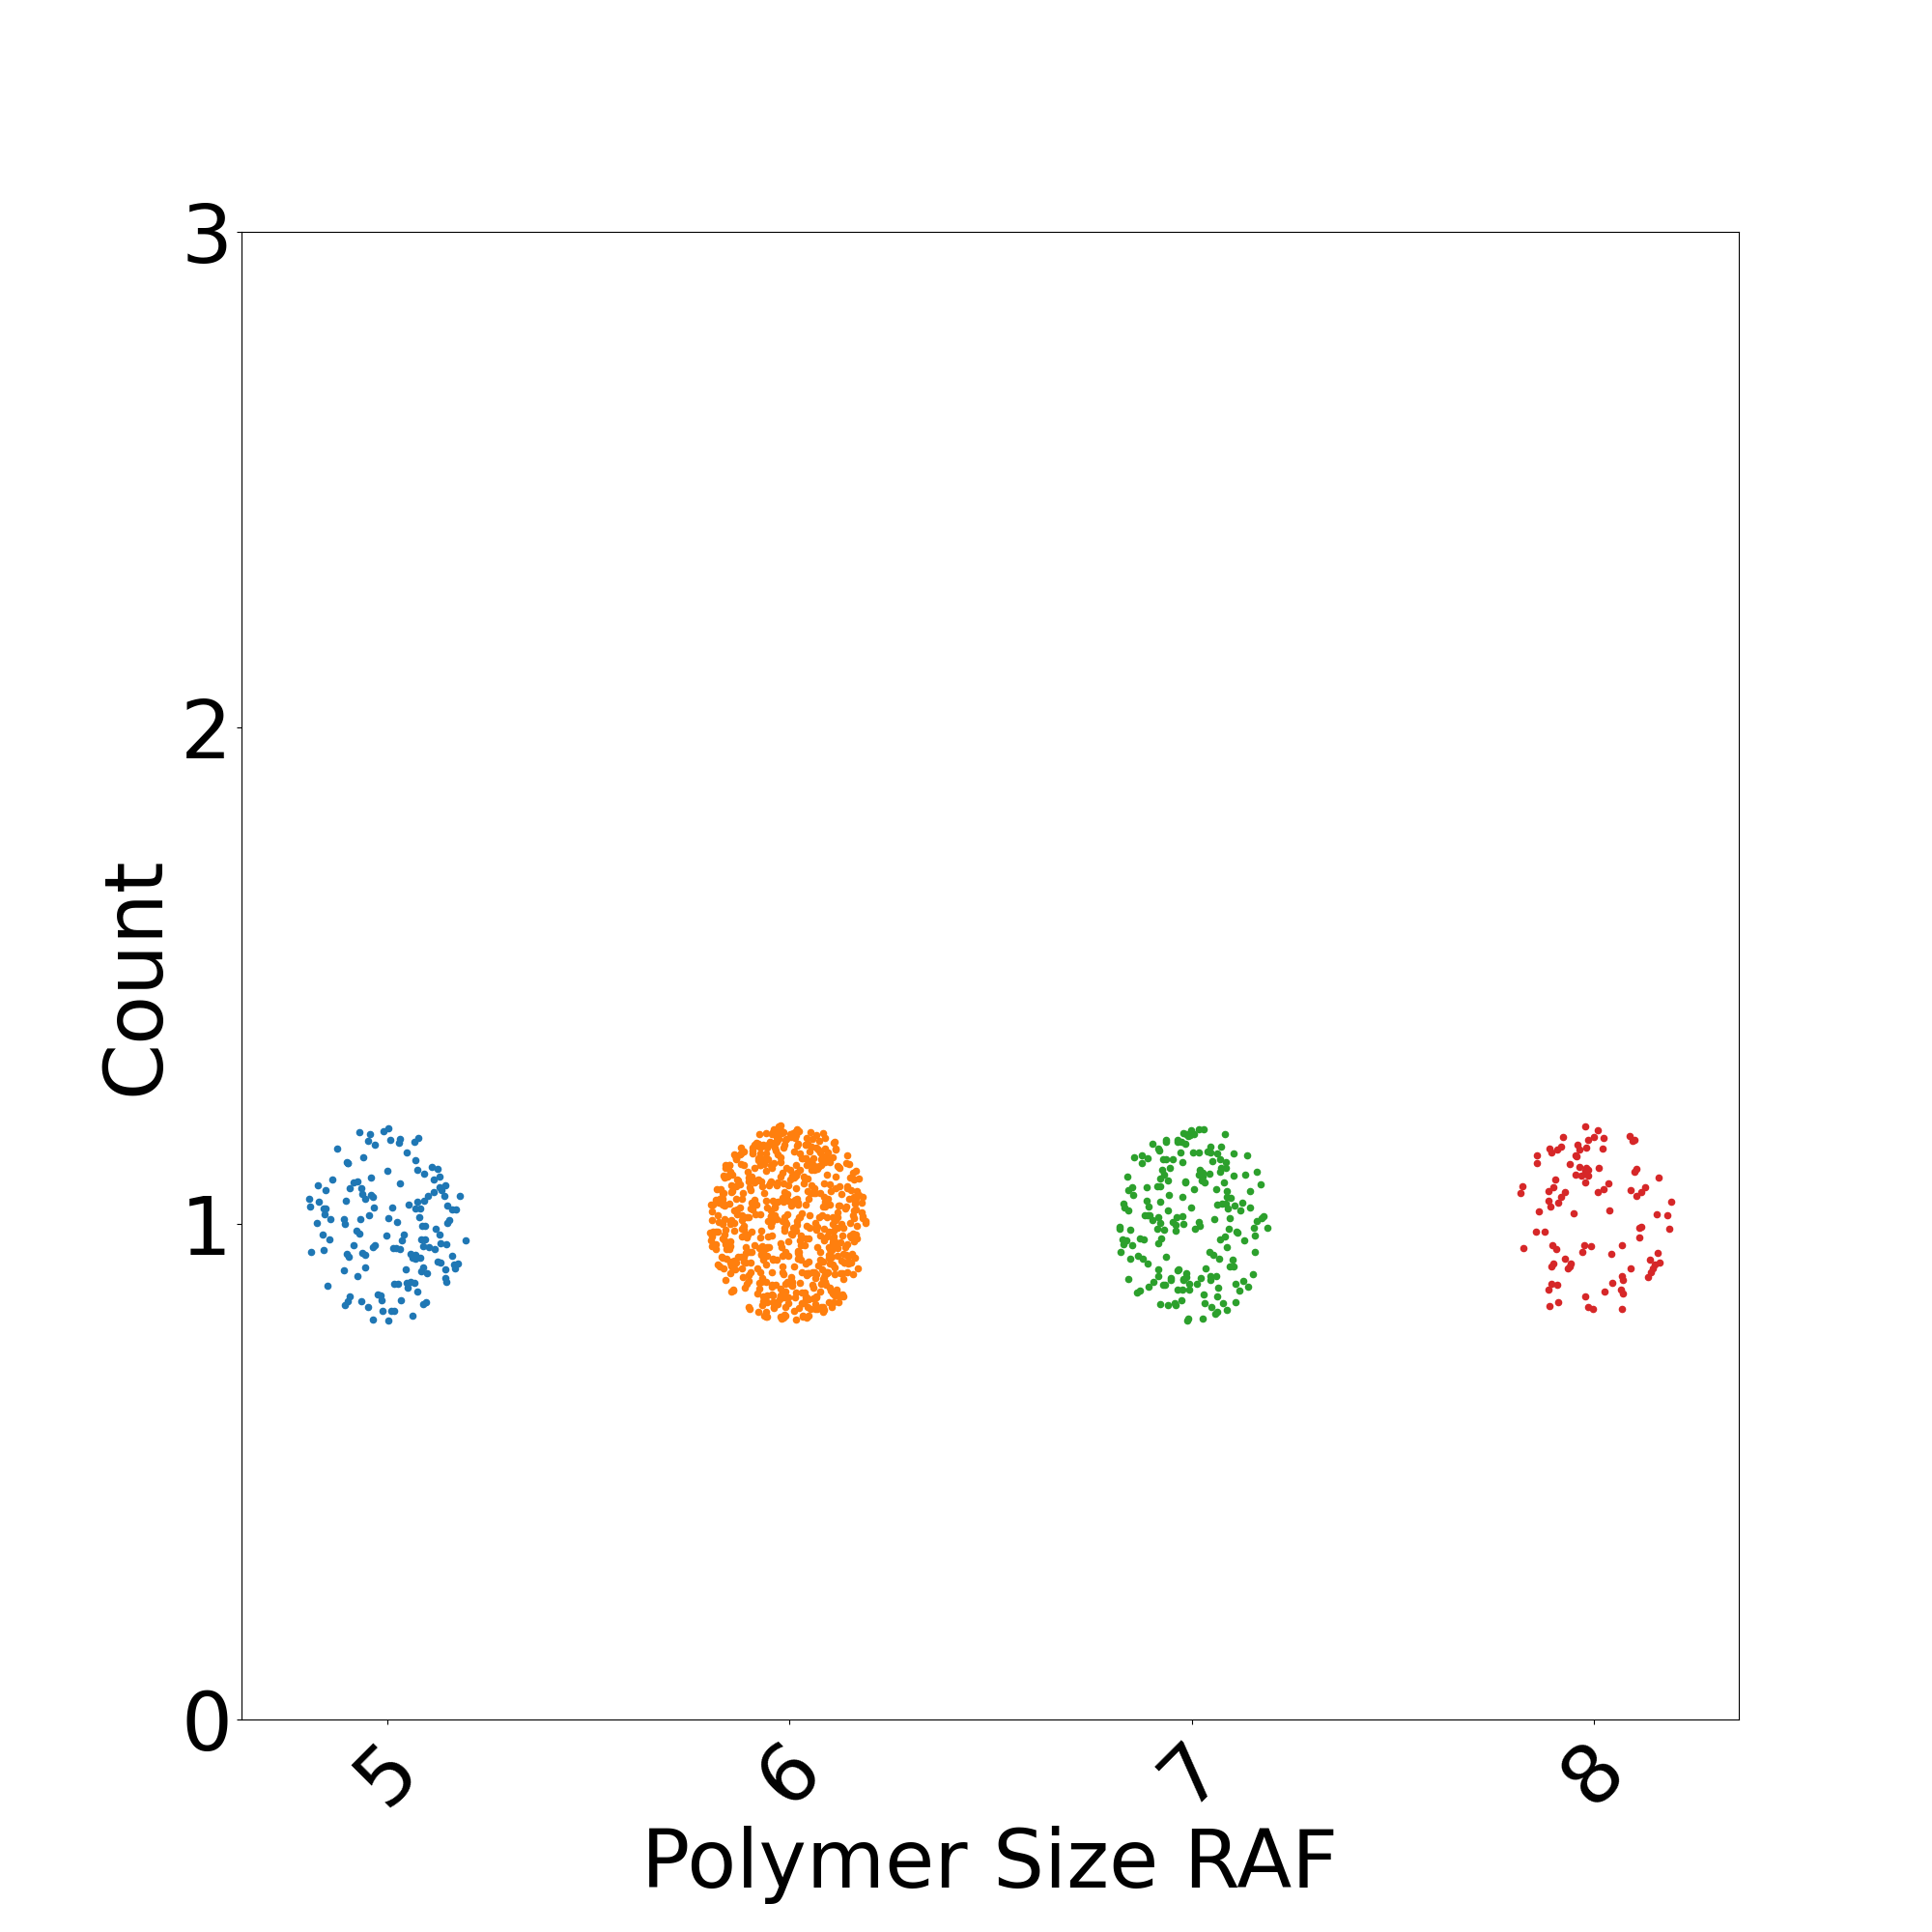
\includegraphics[width=0.8\textwidth]{./Pictures/iRAFirrevStrongBlocks.png}
	\end{minipage}
	\caption{Number of maximal strong blocks containing at least one non-food, 
	non-waste species vertex in irreducible RAFs from different instances of the 
	binary polymer model containing ligation/cleavage (\textbf{left}) or only ligation 
	reactions (\textbf{right}). See SI Table~\ref{tab:SimulationDetails}. Dots, each 
	representing an irreducible RAF with indicated maximal polymer length, are 
	plotted in a non-overlapping manner.} 
	\label{fig:StrongBlocks}
\end{figure}

Figure~\ref{fig:StrongBlocks} shows the number of maximal strong blocks containing at least one non-food, 
non-waste species for all irreducible RAFs collected from the binary polymer models that are specified in 
Tab.~\ref{tab:SimulationDetails}.

Figure~\ref{fig:BPMMultipleStrongBlocks} depicts a theoretical example of an instance of the binary 
polymer model that is composed of two maximal strong blocks containing at least one non-food, 
non-waste species. However, as depicted in Fig.~\ref{fig:StrongBlocks}, such an instance was 
not observed by us. 

\begin{figure}[htb]
	\begin{minipage}[c]{0.4\textwidth}
		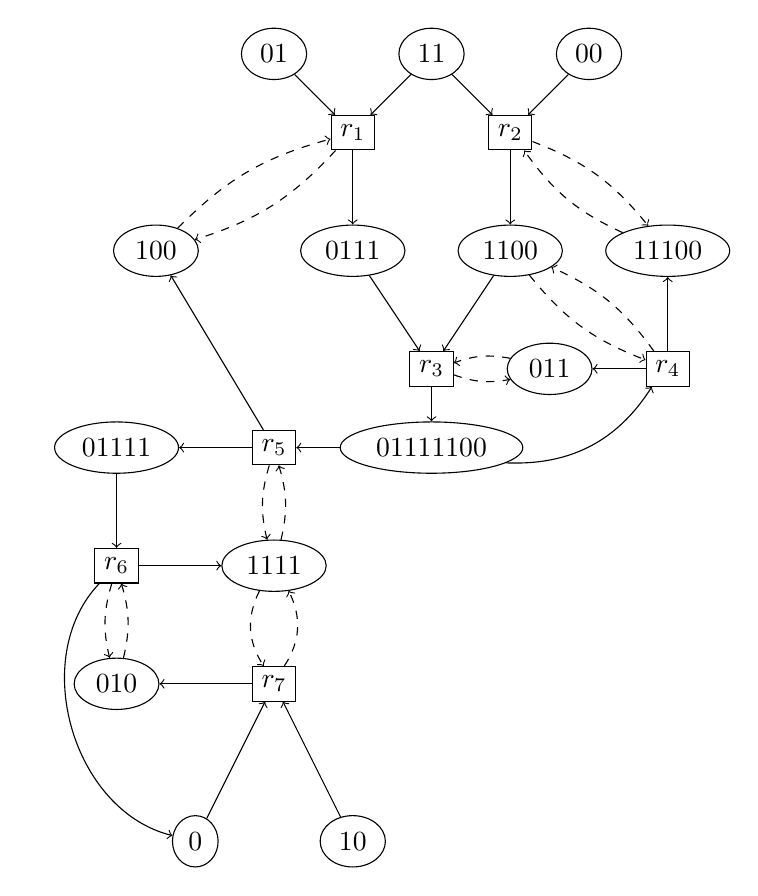
\begin{tikzpicture}
			\node[draw, ellipse] (01) at (0,0) {$01$};
			\node[draw, ellipse] (11) at (2,0) {$11$};
			\node[draw, ellipse] (00) at (4,0) {$00$};						
			\node[draw, ellipse] (100) at (-1.5,-2.5) {$100$};
			\node[draw, ellipse] (0111) at (1,-2.5) {$0111$};
			\node[draw, ellipse] (011) at (3.5,-4) {$011$};
			\node[draw, ellipse] (1100) at (3,-2.5) {$1100$};
			\node[draw, ellipse] (11100) at (5,-2.5) {$11100$};
			\node[draw, ellipse] (01111100) at (2,-5) {$01111100$};
			\node[draw, ellipse] (01111) at (-2, -5) {$01111$};
			\node[draw, ellipse] (1111) at (0, -6.5) {$1111$};
			\node[draw, ellipse] (010) at (-2, -8) {$010$};
			\node[draw, ellipse] (0) at (-1, -10) {$0$};
			\node[draw, ellipse] (10) at (1, -10) {$10$};
			
			\node[draw, rectangle] (r1) at (1,-1) {$r_1$};
			\node[draw, rectangle] (r2) at (3,-1) {$r_2$};
			\node[draw, rectangle] (r3) at (2,-4) {$r_3$};
			\node[draw, rectangle] (r4) at (5,-4) {$r_4$};
			\node[draw, rectangle] (r5) at (0,-5) {$r_5$};
			\node[draw, rectangle] (r6) at (-2,-6.5) {$r_6$};
			\node[draw, rectangle] (r7) at (0,-8) {$r_7$};
			
			\draw[->] (01) to (r1);
			\draw[->] (11) to (r1);
			\draw[->] (r1) to (0111);
			\draw[->, dashed] (100) to [bend left = 15] (r1);
			\draw[->, dashed] (r1) to [bend left = 15] (100);

			\draw[->] (11) to (r2);
			\draw[->] (00) to (r2);			
			\draw[->] (r2) to (1100);
			\draw[->, dashed] (11100) to [bend left = 15] (r2);
			\draw[->, dashed] (r2) to [bend left = 15] (11100);
			
			\draw[->] (0111) to (r3);
			\draw[->] (1100) to (r3);
			\draw[->, dashed] (r3) to [bend right = 15] (011);
			\draw[->, dashed] (011) to [bend right = 15] (r3);
			\draw[->] (r3) to (01111100);
			
			\draw[->] (01111100) to [bend right = 30] (r4);
			\draw[->] (r4) to (11100);
			\draw[->] (r4) to (011);
			\draw[->, dashed] (r4) to [bend right = 15] (1100);
			\draw[->, dashed] (1100) to [bend right = 15] (r4);
			
			\draw[->] (01111100) to (r5);
			\draw[->] (r5) to (100);
			\draw[->] (r5) to (01111);
			\draw[->, dashed] (r5) to [bend right = 15] (1111);
			\draw[->, dashed] (1111) to [bend right = 15] (r5);
			
			\draw[->] (01111) to (r6);
			\draw[->] (r6) to (1111);
			\draw[->] (r6) to [bend right = 60] (0);
			\draw[->, dashed] (r6) to [bend right = 15] (010);
			\draw[->, dashed] (010) to [bend right = 15] (r6);
			
			\draw[->] (0) to (r7);
			\draw[->] (10) to (r7);
			\draw[->] (r7) to (010);
			\draw[->, dashed] (r7) to [bend right = 30] (1111);
			\draw[->, dashed] (1111) to [bend right = 30] (r7);
		\end{tikzpicture}
	\end{minipage}%
	\hfill%
	\begin{minipage}[c]{0.6\textwidth}
		\par\bigskip
		\par\bigskip
		\par\bigskip
		\par\bigskip
		\par\bigskip
		\par\bigskip
		\par\bigskip
		\par\bigskip
		\par\bigskip
		\par\bigskip
		\par\bigskip
		\par\bigskip
		\begin{equation*}
			\begin{split}
				r_1&: 01 + 11 + (100) \rightarrow 0111 + (100) \\
				r_2&: 11 + 00 + (11100) \rightarrow 1100 + (11100) \\
				r_3&: 0111 + 1100 (011) \rightarrow 01111100 + (011) \\
				r_4&: 01111100 + (1100) \rightarrow 011 + 11100 + (1100) \\
				r_5&: 01111100 + (1111) \rightarrow 01111 + 100 + (1111) \\
				r_6&: 01111 + (010) \rightarrow 0 + 1111 + (010) \\
				r_7&: 0 + 10 + (1111) \rightarrow 010 + (1111)
			\end{split}
		\end{equation*}
	\end{minipage}
	\caption{Example for an irreducible RAF from the binary polymer model with multiple strong blocks.}
	\label{fig:BPMMultipleStrongBlocks}	
\end{figure}

\subsection{Compositions of irreducible RAFs}

Figure~\ref{fig:irrRAFCoreComp} shows the composition in terms of F-reactions of the 50 arbitrarily chosen 
irreducible RAFs from two instances of the binary polymer model, i.e., n6\_split and n6\_forw, depicted in 
Fig.~\ref{M-fig:irrRAFCores}.

\begin{figure}
	\centering
	\begin{minipage}[c]{0.5\textwidth}
		\centering
		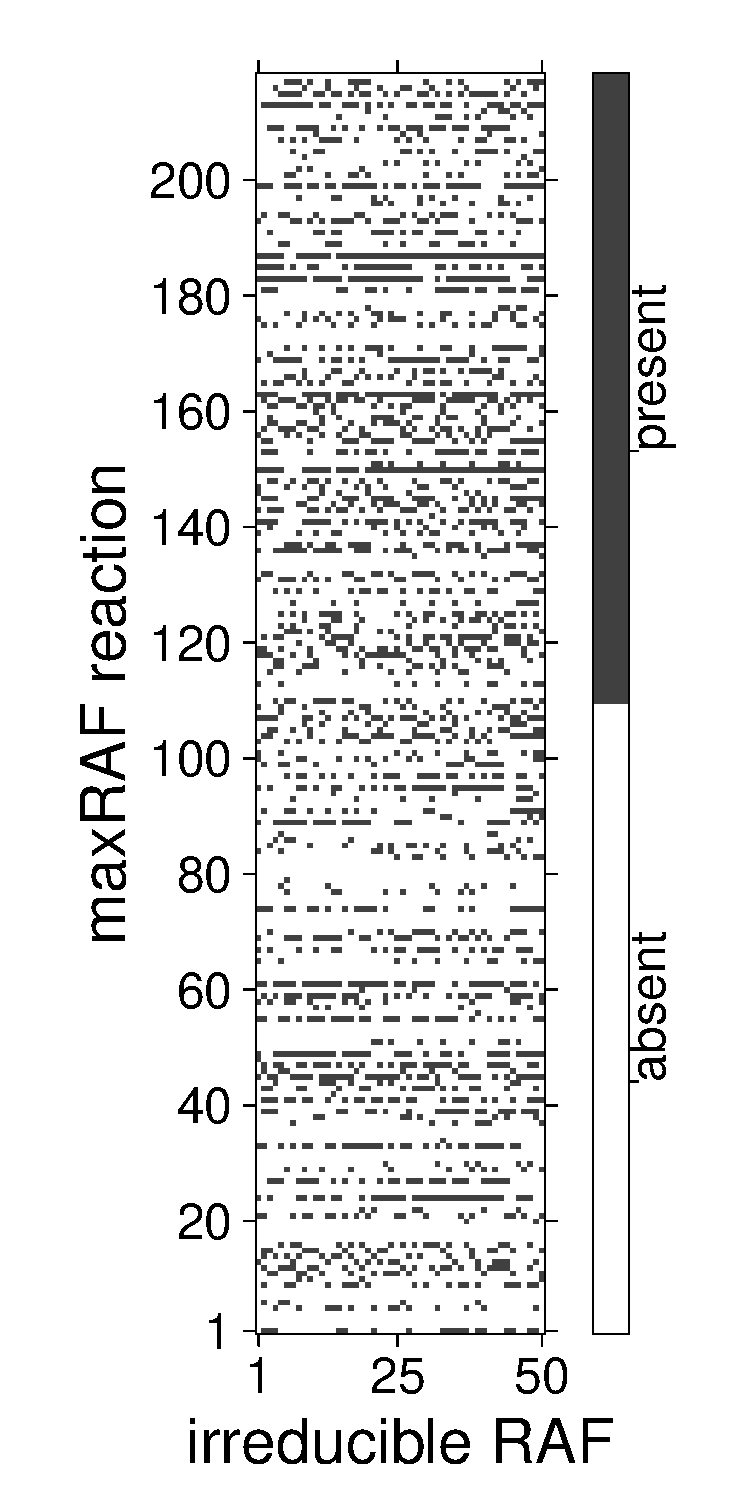
\includegraphics[width=\textwidth]{./Pictures/n6_split_present.pdf}
	\end{minipage}%
	\hfill%
	\begin{minipage}[c]{0.5\textwidth}
		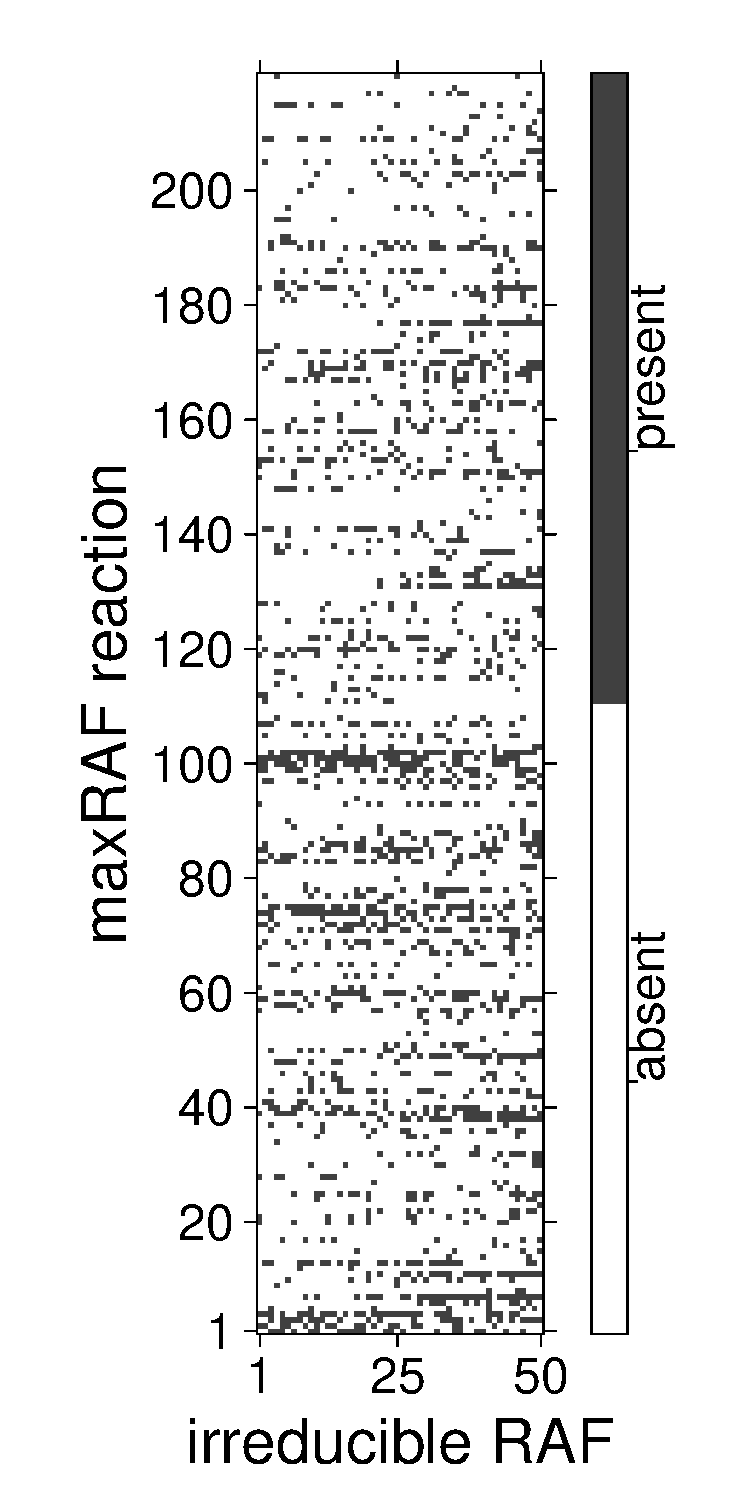
\includegraphics[width=\textwidth]{./Pictures/n6_forw_present.pdf}
	\end{minipage}
	\caption{Depiction of the F-reaction composition of 50 arbitrarily chosen 
	irreducible RAFs from two instances of the binary polymer model as depicted in 
	Fig.~\ref{M-fig:irrRAFCores} with maximal polymer size of $n=6$. See  
	Table~\ref{tab:SimulationDetails} for simulation details.}
	\label{fig:irrRAFCoreComp}
\end{figure}



\end{document}
